\subsubsection{Multilayer Feedworward Networks} 
\label{sec:theory-multilayer} 

We will define \emph{multilayer feedforward networks} as in \citet{haykin1994neural}. First, we define a \emph{layered} neural network where neurons are organised to form layers. In the simplest version we have an \emph{input layer} of source nodes and an \emph{output layer} which is formed by aforementioned perceptrons. In other words this is a \emph{feedforward} or \emph{acyclic} type of network as the \emph{activation}, i.e. outputs of the neurons are computed from the input to the output layer and never \emph{backwards}. 

Multilayer neural network has one or more \emph{hidden layers} in addition to the input and ouput layer as shown on figure~\ref{fig:multilayer}. The source nodes supply the activation pattern, i.e. input vector, which is applied to second layer neurons. The output signal of the hidden layer is used as the input for the output layer. As shown by \citet{cybenko1989approximation} the three layer network is an universal approximator continuous functions on compact subsets of $\mathbb{R}^n$.

\begin{figure}[H]
  \centering
  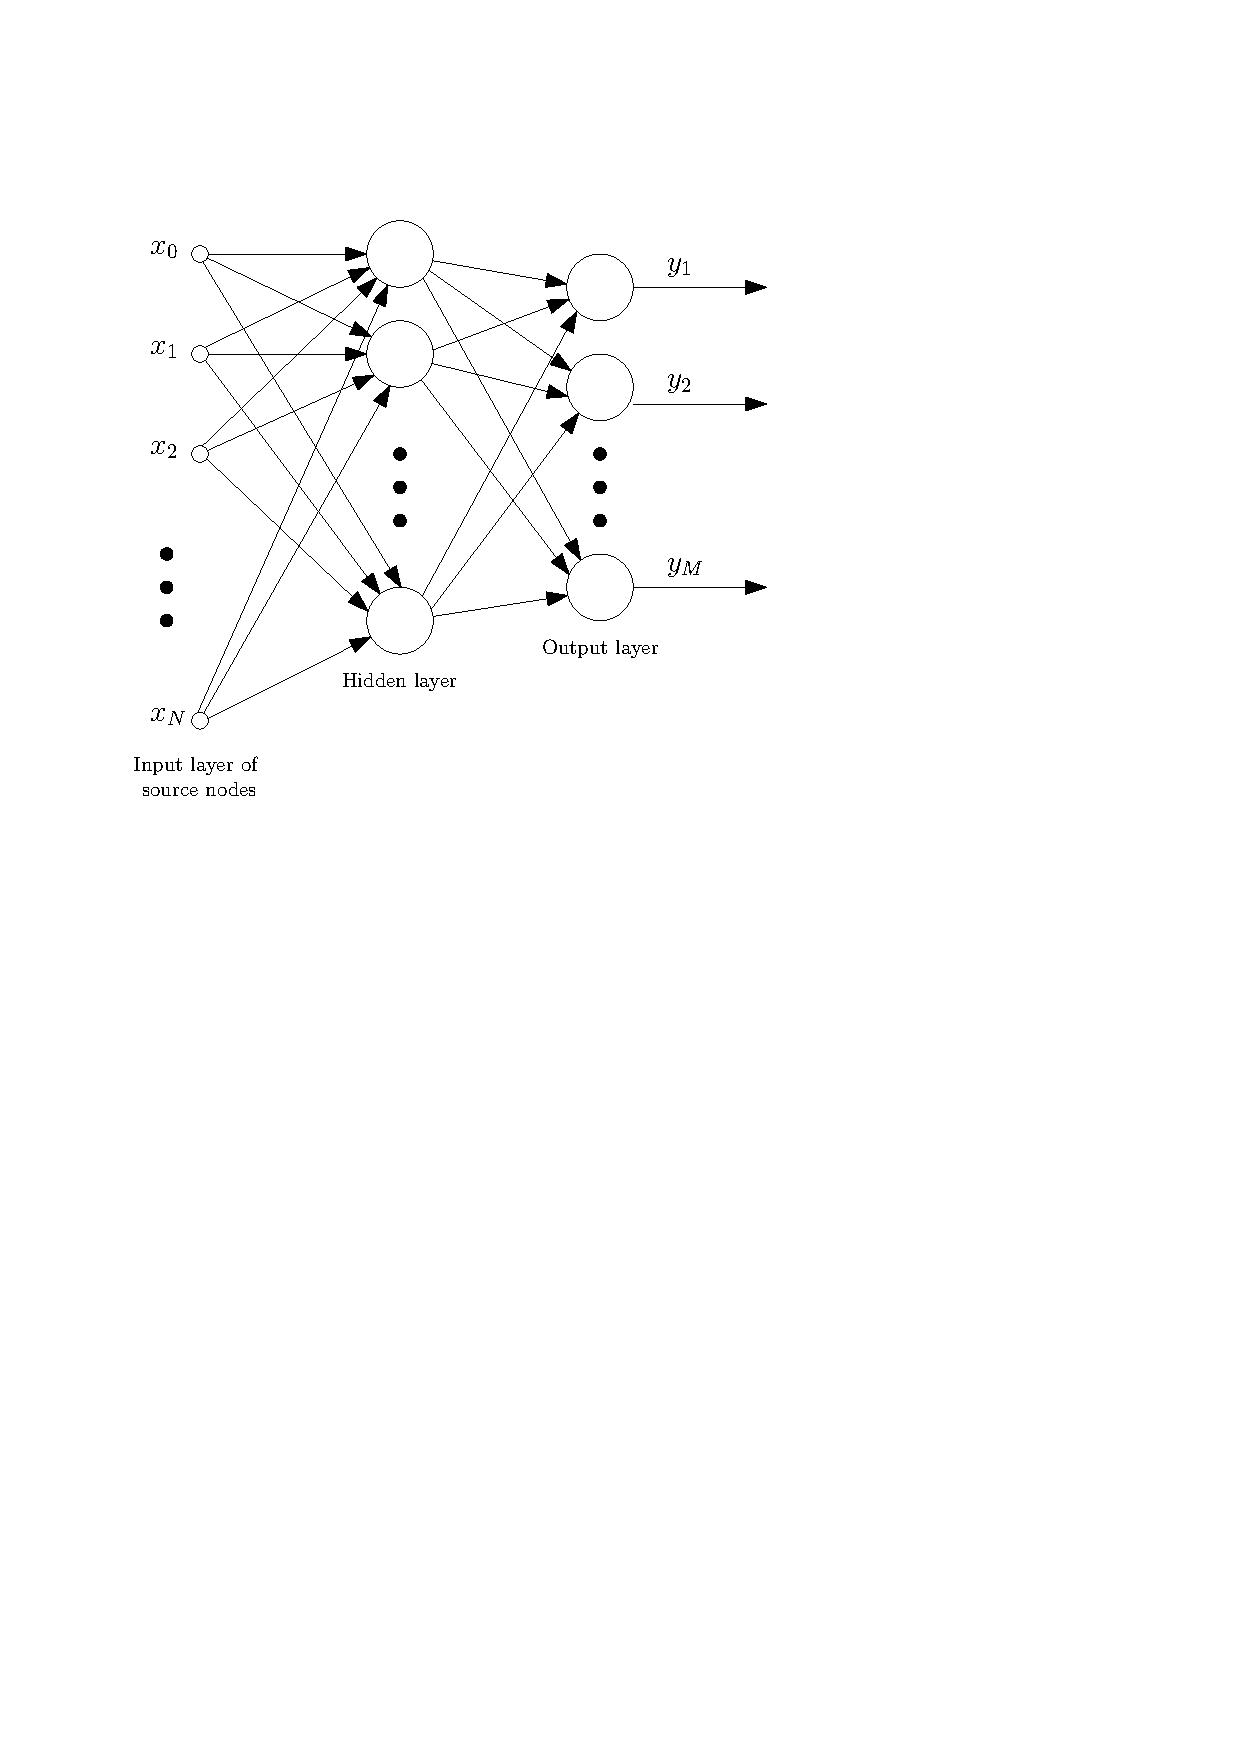
\includegraphics[width=0.5\textwidth]{img/multilayer.pdf}    
  \caption{Fully connected feedforward \emph{multilayer} network with one \emph{hidden} layer and one \emph{output} layer. } 
  \label{fig:multilayer}
\end{figure}

There exists several methods for training multilayer networks. First, we will describe the most common Backpropagation in (\ref{sec:models-bp}) and then methods related to our work such as CHL (\ref{sec:models-chl}), GeneRec (\ref{sec:models-generec}) and BAL (\ref{sec:models-bal}). 
